\documentclass{standalone}
\author{Quinten Bruynseraede}
\usepackage{tikz}
\usetikzlibrary{shapes}
\title{Tikz grafen}
\begin{document}\pagestyle{empty}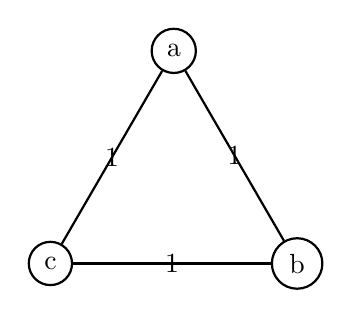
\begin{tikzpicture}\node[shape=circle,draw=black,align=center,line width=0.8pt] (0) at (6.233333333333333,13.066666666666666) {a};
\node[shape=circle,draw=black,align=center,line width=0.8pt] (1) at (4.666666666666667,10.366666666666667) {c};
\node[shape=circle,draw=black,align=center,line width=0.8pt] (2) at (7.8,10.366666666666667) {b};

\path [-,draw=black,line width=0.8pt] (1) edge node {1} (0);
\path [-,draw=black,line width=0.8pt] (0) edge node {1} (2);
\path [-,draw=black,line width=0.8pt] (2) edge node {1} (1);
\end{tikzpicture}
\end{document}